% ==================================================================
%  Short seminar version: circuit -> current vs coupling -> microscopic model -> phase diagram
%  Build: cd talk && pdflatex talk_short.tex (twice).  Figures: ../figs/*, figs/* (make_talk_figs.py, make_short_figs.py)
% ==================================================================
\documentclass[aspectratio=169,10pt]{beamer}
\usetheme[progressbar=frametitle,numbering=fraction,block=fill]{metropolis}
\usepackage[T1]{fontenc}
\usepackage{lmodern}
\usepackage{amsmath,amssymb,bm,mathtools}
\usepackage{booktabs}
\usepackage{tikz}
\usetikzlibrary{arrows.meta,positioning,calc}
\usepackage[american]{circuitikz}
\usepackage[most]{tcolorbox}
\usepackage{appendixnumberbeamer}

\definecolor{ink}{HTML}{1F2A44}
\definecolor{accent}{HTML}{2A6FDB}
\definecolor{warm}{HTML}{E8692B}
\definecolor{good}{HTML}{1AA37A}
\definecolor{paper}{HTML}{FAFAF7}
\definecolor{purp}{HTML}{5B3FA8}
\setbeamercolor{normal text}{fg=ink,bg=paper}
\setbeamercolor{alerted text}{fg=warm}
\setbeamercolor{frametitle}{bg=ink,fg=white}
\setbeamercolor{progress bar}{fg=warm,bg=ink!30}
\setbeamertemplate{itemize items}{\color{accent}$\blacktriangleright$}
\newtcolorbox{keybox}[1][]{enhanced,colback=accent!6,colframe=accent,boxrule=0.8pt,arc=2mm,
  left=2mm,right=2mm,top=1mm,bottom=1mm,before upper=\raggedright,#1}
\newtcolorbox{warnbox}[1][]{enhanced,colback=warm!7,colframe=warm,boxrule=0.8pt,arc=2mm,
  left=2mm,right=2mm,top=1mm,bottom=1mm,before upper=\raggedright,#1}

\newcommand{\hw}{\hbar\omega}
\newcommand{\Hring}{H_{\rm ring}}
\newcommand{\pcl}{\varphi_{\rm cl}}
\newcommand{\cw}{\circlearrowright}
\newcommand{\ccw}{\circlearrowleft}
\renewcommand{\cite}[1]{{\scriptsize\textcolor{ink!60}{[#1]}}}
\graphicspath{{../figs/}{figs/}}

\title{A $\pi$ loop coupled to a quantum $LC$ circuit: spontaneous persistent current, exactly}
\subtitle{From the rf-SQUID circuit model to a quantum-dot Josephson loop solved by DMRG}
\author{Group seminar}
\date{}

\begin{document}

\begin{frame}[plain]
  \titlepage
\end{frame}

% ==================================================================
\section{The circuit}

\begin{frame}{The circuit: an rf-SQUID and a detached $LC$ circuit}
  \begin{columns}[c]
    \column{0.5\textwidth}
    \centering
    \begin{circuitikz}[scale=0.95,transform shape]
      % LC circuit
      \draw[blue!70!black,line width=1.1pt] (0,0) to[C,l_=$C_r$] (0,2.4) -- (1.5,2.4) to[L,l_=$L_c$] (1.5,0) -- (0,0);
      \node[blue!70!black] at (0.75,2.9) {$\hbar\omega_r\,a^\dagger a$};
      % mutual
      \draw[<->,dashed,thick,purp] (1.75,0.45) -- (2.95,0.45) node[midway,above,purp] {$M$};
      % SQUID loop
      \draw[line width=1.6pt] (3.2,0) to[L,l=$L_r$] (3.2,2.4) -- (5.4,2.4) -- (5.4,1.6);
      \draw[line width=1.6pt] (5.4,0.8) -- (5.4,0) -- (3.2,0);
      \draw[thick,fill=white] (5.1,0.8) rectangle (5.7,1.6);
      \draw[thick] (5.1,0.8) -- (5.7,1.6); \draw[thick] (5.1,1.6) -- (5.7,0.8);
      \node[right] at (5.75,1.45) {$E_J$};
      \node[right] at (5.75,0.95) {$E_C$};
      \draw[-{Stealth[length=2.5mm]},thick,ink!70] (4.75,1.7) arc (60:120:0.8);
      \draw[-{Stealth[length=2.5mm]},thick,ink!70] (3.95,0.7) arc (240:300:0.8);
      \node at (4.35,1.2) {$\pm I$};
      \node at (4.3,2.9) {$\varphi,\ N$};
    \end{circuitikz}
    \column{0.5\textwidth}
    \begin{itemize}
      \item \textbf{Loop:} a Josephson junction ($E_J$, charging energy $E_C$) closing an inductance $L_r$
            ($E_L$). Biased at half a flux quantum, $\varphi_{\rm ext}=\pi$ -- or closed by an intrinsic $\pi$ junction --
            it is a \alert{$\pi$ loop}.
      \item \textbf{$LC$ circuit}, galvanically detached, mode $a$ at $\omega_r$: its flux $MI_c\propto a+a^\dagger$ threads the loop.
      \item No current drive, only a seed $\varphi_{\rm ext}=\pi-10^{-3}$ to pick a direction.
    \end{itemize}
    \begin{keybox}
      \textbf{Question:} does the quantum flux of the $LC$ circuit make the loop carry a persistent current?
    \end{keybox}
  \end{columns}
\end{frame}

% ------------------------------------------------------------------
\begin{frame}{The two-mode Hamiltonian (original notebook)}
  \vspace{-1mm}
  {\small\[
    H=E_C\,N^2+E_L\big(\varphi-\varphi_{\rm ext}-g\,(a+a^\dagger)\big)^2-E_J\cos\varphi+\hbar\omega_r\,a^\dagger a,
    \qquad \varphi=\tfrac{1}{\sqrt2}\big(\tfrac{E_C}{E_L}\big)^{1/4}(b+b^\dagger),\ \ [\varphi,N]=i
  \]}
  \vspace{-4mm}
  \begin{columns}[T]
    \column{0.5\textwidth}
    \begin{keybox}[title={Resonator seen statically (minimize over $a+a^\dagger$)}]
      \footnotesize $\dfrac{1}{E_L^{\rm eff}}=\dfrac{1}{E_L}+\dfrac{4g^2}{\hbar\omega_r}$: the $LC$ circuit \emph{adds inductance}
      to the loop ($M^2/L_c$).\ Screening parameter
      $\beta_{\rm eff}=\dfrac{E_J}{2E_L^{\rm eff}}=\dfrac{E_J}{2E_L}(1+4g_1^2)$, $g_1^2\equiv g^2E_L/\hbar\omega_r$:
      the only combination the static problem knows.
    \end{keybox}
    \footnotesize Notebook ($E_C=1$): $E_L=0.5$, $E_J=2$: $\beta_{\rm loop}=2$, but the bare well ($0.84E_C$) lies below
    $\omega_{rf}=2\sqrt{E_CE_L}=1.4$ -- no polarization without the resonator.
    \column{0.5\textwidth}
    \begin{keybox}[title={Mean field of the notebook: $|{\rm GS}\rangle=|\psi_{rf}\rangle|\psi_{ph}\rangle$}]
      \footnotesize Resonator in a coherent state $\alpha\propto\langle\varphi\rangle$, SQUID mode $b$ exact (200 Fock states):
      \[
        H^{\rm mf}_{rf}=E_CN^2+E_L\varphi^2-E_J\cos\varphi-\frac{2E_Lg_1^2}{\tfrac14+g_1^2}\,\langle\varphi\rangle\,\varphi
      \]
      ($\varphi\to\varphi-\varphi_{\rm ext}$), self-consistent in $\langle\varphi\rangle$ = Hartree linearization of the exact
      static term. The resonator's zero-point motion is gone: mean field depends on $g_1$ only, the exact problem on $g$ and $\omega_r$.
    \end{keybox}
  \end{columns}
\end{frame}

% ------------------------------------------------------------------
\begin{frame}{What the notebook predicts, and what the exact two-mode solution says}
  \centering
  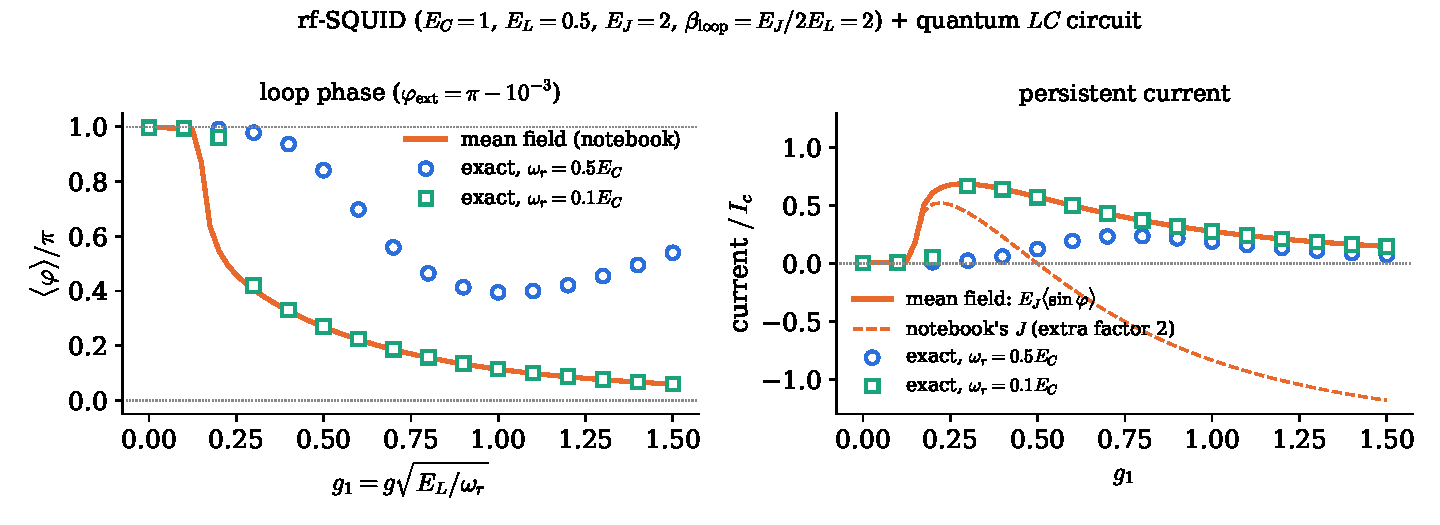
\includegraphics[width=0.8\textwidth]{rfsquid_mf.pdf}
  \begin{columns}[T]
    \column{0.5\textwidth}
    \footnotesize Mean field (reproduced to all digits): the loop polarizes at $g_1\simeq0.15$--$0.3$, the current peaks at
    $0.69\,I_c$ and then falls as the loop lets in half a flux quantum ($\langle\varphi\rangle\to0$).
    \alert{Caveat:} the notebook evaluates $J$ with $(1-2c)$ instead of $(1-c)$, $c=g_1^2/(\frac14+g_1^2)$;
    the correct $-\partial E/\partial\varphi_{\rm ext}$ equals $E_J\langle\sin\varphi\rangle$ (solid).
    \column{0.5\textwidth}
    \footnotesize Exact ground state of both modes (seed $10^{-3}$): for a slow resonator ($\omega_r=0.1E_C$) it follows the
    mean field; for $\omega_r=0.5E_C$ the state stays a \alert{cat} and the current is $\le0.24\,I_c$.
    Zero-point motion of the resonator opposes the polarization -- exactly what the microscopic model will show.
  \end{columns}
\end{frame}

% ------------------------------------------------------------------
\begin{frame}{The limit we then solve exactly: loop flux locked to the $LC$ flux}
  \begin{columns}[T]
    \column{0.52\textwidth}
    \small Take $E_L\to\infty$ ($k=M/\sqrt{L_rL_c}\to1$): $E_L(\varphi-g(a+a^\dagger))^2$ locks $\varphi=g(a+a^\dagger)$ and the
    loop mode $b$ ($\omega_{rf}\to\infty$) freezes out:
    \begin{keybox}
      \centering$\displaystyle H\;\to\;\hbar\omega\,a^\dagger a+E_J\cos\!\big[2g\,(a+a^\dagger)\big]$
    \end{keybox}
    \footnotesize for a $\pi$ junction ($+E_J\cos$; $2g$ = pair-phase coupling, $g^2=\pi Z/4R_Q$). This is the circuit of the
    manuscript: the loop \emph{is} the inductor of the mode (fluxonium-like, galvanic). In the pair phase $\theta=2gX$:
    \[
      H=4E_C\,n^2+\tfrac12E_L\theta^2+E_J\cos\theta,\quad E_L=\frac{\hbar\omega}{8g^2},\ E_C=\hbar\omega g^2,
    \]
    \footnotesize $\beta=E_J/E_L=8g^2E_J/\hbar\omega=2\pi LI_c/\Phi_0$: the $4g_1^2$ term of the two-mode model alone.
    \column{0.46\textwidth}
    \begin{keybox}[title={Why this limit}]
      \footnotesize It keeps the mechanism (the resonator's inductance and zero-point flux act on the junction) with one
      bosonic mode, so that the junction can be replaced by the \emph{microscopic} interacting ring and solved by DMRG.
    \end{keybox}
    \begin{warnbox}[title={What the inductive case ($k<1$) adds}]
      \footnotesize Same classical threshold ($L\to L_r^{\rm total}$) and cat physics, but two zero-point fluxes sharing
      $\delta$, the photon numbers and the flux-driven $0$--$\pi$ shift: a second bosonic site in the DMRG, not yet computed.
    \end{warnbox}
  \end{columns}
\end{frame}

% ------------------------------------------------------------------
\begin{frame}{Classical picture: a double well and a pitchfork}
  \centering
  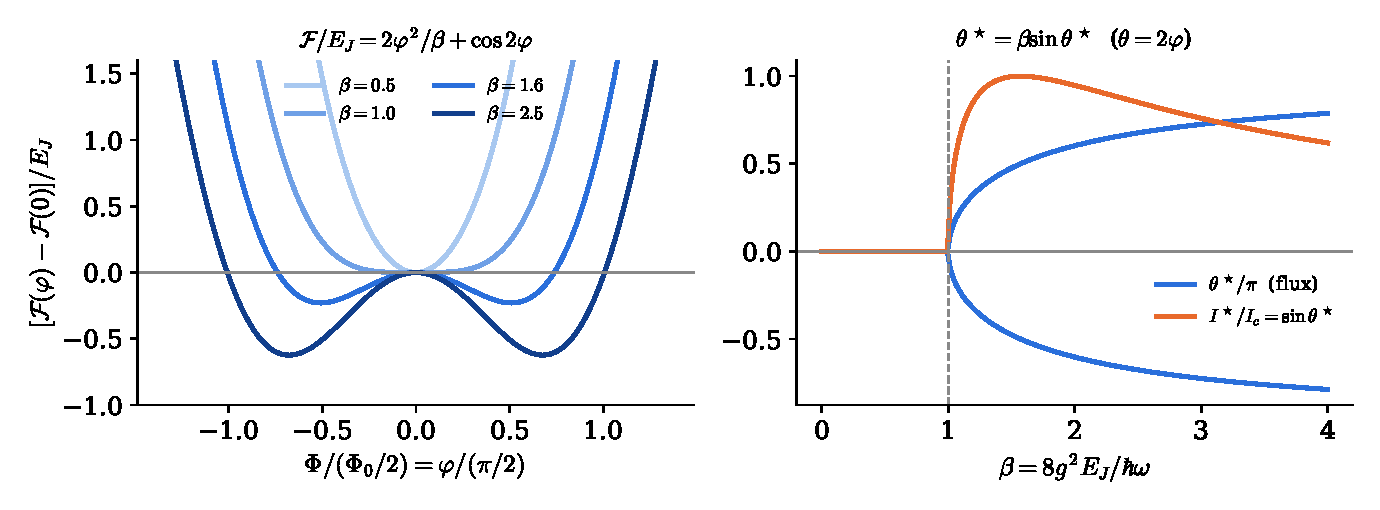
\includegraphics[width=0.9\textwidth]{landau.pdf}
  \par\vspace{1mm}
  Minima at $\theta^\star=\beta\sin\theta^\star$ carry the current $I^\star=I_c\sin\theta^\star$ and a static flux
  $\langle\Phi\rangle=LI^\star$: a ``photon condensate'' $\langle a\rangle\neq0$.
  The exact identity $\langle I\rangle=\langle\Phi\rangle/L$ holds in every quantum eigenstate.
\end{frame}

% ------------------------------------------------------------------
\begin{frame}{The persistent current that emerges}
  \centering
  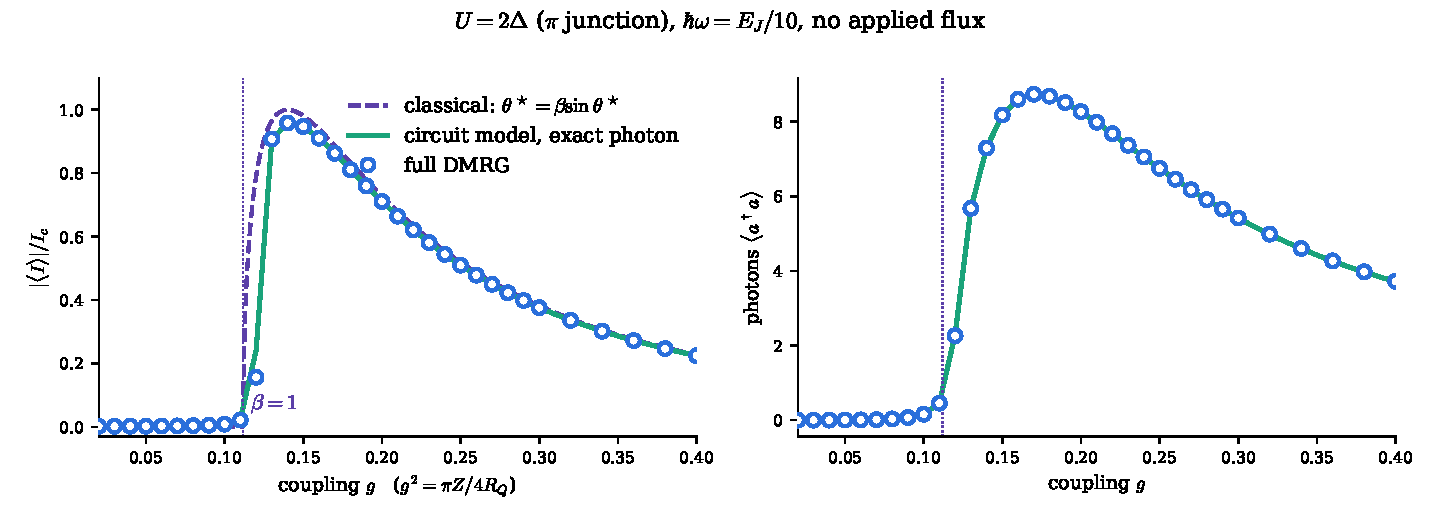
\includegraphics[width=0.84\textwidth]{current_vs_g.pdf}
  \begin{itemize}\small
    \item Above $g_c\simeq0.13$: a current of $0.96\,I_c$ and a condensate of $7$--$9$ photons. The threshold lies slightly
          \alert{above} the classical $\beta=1$; beyond it the current falls as $\hw/g^2$ (the flux saturates at $\Phi_0/2$).
    \item Circles: full microscopic solution (next part); line: circuit Hamiltonian with an exact photon -- they agree to $0.2\%$ of $I_c$.
  \end{itemize}
\end{frame}

% ------------------------------------------------------------------
\begin{frame}{What is the quantum ground state? A cat}
  \centering
  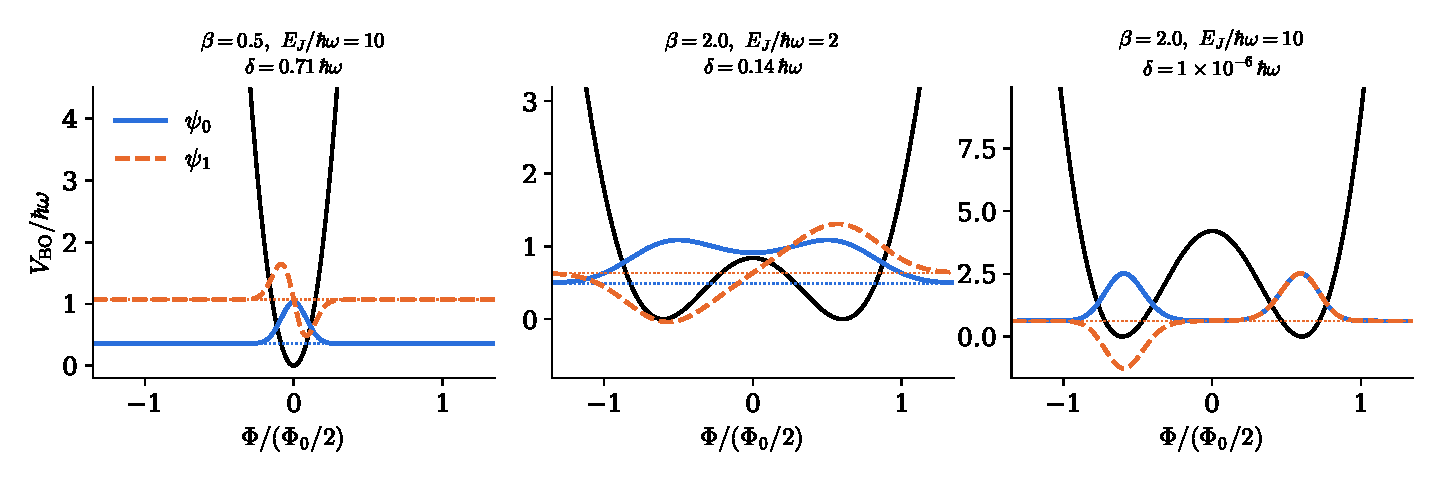
\includegraphics[width=0.85\textwidth]{quantum_well.pdf}
  \begin{columns}[T]
    \column{0.55\textwidth}
    \small Exact eigenstates of the circuit Hamiltonian. For $\beta>1$ the ground state is the symmetric superposition
    $(|\cw\rangle+|\ccw\rangle)/\sqrt2$ of the two current directions, split from its partner by a tunnel gap
    $\delta\sim\hw\,e^{-(E_J/\hw)\,s(\beta)}$.
    \column{0.45\textwidth}
    \small A tiny flux offset ($\delta\Phi>\delta/2I^\star$) selects one direction. If $E_J\lesssim\hw$ the well is
    shallower than the zero-point energy and no current state exists at all (middle panel).
  \end{columns}
\end{frame}

% ==================================================================
\section{Where does \texorpdfstring{$E_J\cos\theta$}{EJ cos theta} come from? The microscopic model}

\begin{frame}{The microscopic model: a quantum dot in a BCS ring, plus the mode}
  \vspace{-3mm}
  \begin{align*}
    H={}&\textcolor{blue!70!black}{\hw\,a^\dagger a}
      \;\underbrace{-\,t\sum_{r,\sigma}\big(c^\dagger_{r+1\sigma}c_{r\sigma}+\text{h.c.}\big)
      +\Delta\sum_{r}\big(c^\dagger_{r\uparrow}c^\dagger_{r\downarrow}+\text{h.c.}\big)}_{\text{BCS ring, }L-1\text{ sites}}
      +\underbrace{\epsilon_d\,n_0+\textcolor{warm}{U\,n_{0\uparrow}n_{0\downarrow}}}_{\text{Anderson dot}}\\
     &-\,t_J\sum_\sigma\big(c^\dagger_{0\sigma}c_{L-1\,\sigma}+\text{h.c.}\big)
      -t_J\sum_\sigma\Big(\textcolor{blue!70!black}{e^{ig(a+a^\dagger)}}\,c^\dagger_{1\sigma}c_{0\sigma}+\text{h.c.}\Big)
  \end{align*}
  \begin{columns}[T]
    \column{0.55\textwidth}
    \begin{itemize}\small
      \item The flux is a Peierls phase on the dot bond; quantized, it becomes the displacement operator
            $e^{ig(a+a^\dagger)}$ (diamagnetic terms to all orders).
      \item Parity is conserved: \textbf{even} = singlet, a $0$ junction; \textbf{odd} = Kramers doublet, a $\pi$ junction
            (a Cooper pair crosses the singly occupied dot with its spins reversed).
    \end{itemize}
    \column{0.45\textwidth}
    \begin{keybox}
      \small Solved \alert{exactly} by DMRG on the full electron$\otimes$photon space ($\chi=300$, Fock cutoff $50$--$60$,
      sum rule $\langle I\rangle=\langle\Phi\rangle/L$ as acceptance test).\\[1mm]
      $\Delta=t$, $t_J=0.5\Delta$, $\epsilon_d=-U/2$, $L=10$, $\hw=E_J(2\Delta)/10$.
    \end{keybox}
  \end{columns}
\end{frame}

% ------------------------------------------------------------------
\begin{frame}{The junction alone: $0$ or $\pi$ is decided by $U$}
  \centering
  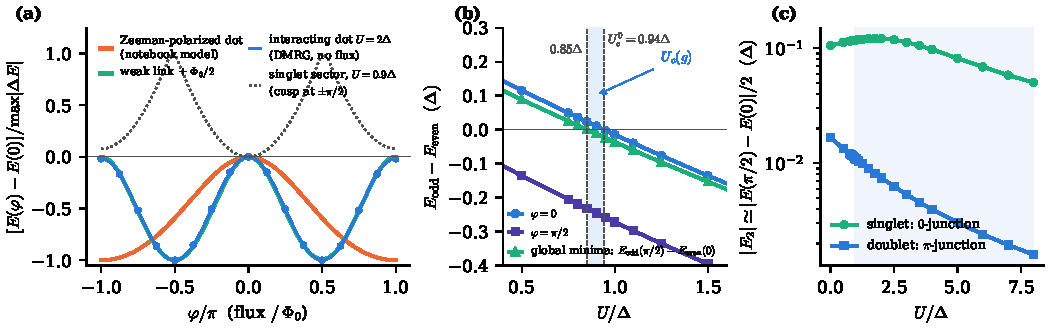
\includegraphics[width=0.95\textwidth]{fig_junctions.pdf}
  \begin{columns}[T]
    \column{0.5\textwidth}
    \small (a) Ring energy vs flux. The doublet at $U=2\Delta$ is a pure $\pi$ junction, $E_2=7.39\times10^{-3}\Delta$;
    at zero flux it looks exactly like an ordinary weak link biased by $\Phi_0/2$.
    \column{0.5\textwidth}
    \small (b) Singlet--doublet crossing at $U_c^0=0.94\Delta$ (zero flux); the \emph{global} minima cross already at $0.85\Delta$.
    (c) $E_J$ of the $\pi$ junction falls as $U^{-1.3}$: $E_J/\hw$ runs from $15$ to $2$ across the phase diagram.
  \end{columns}
\end{frame}

% ==================================================================
\section{The phase diagram}

\begin{frame}{Phase diagram in the $(U,g)$ plane -- full DMRG}
  \centering
  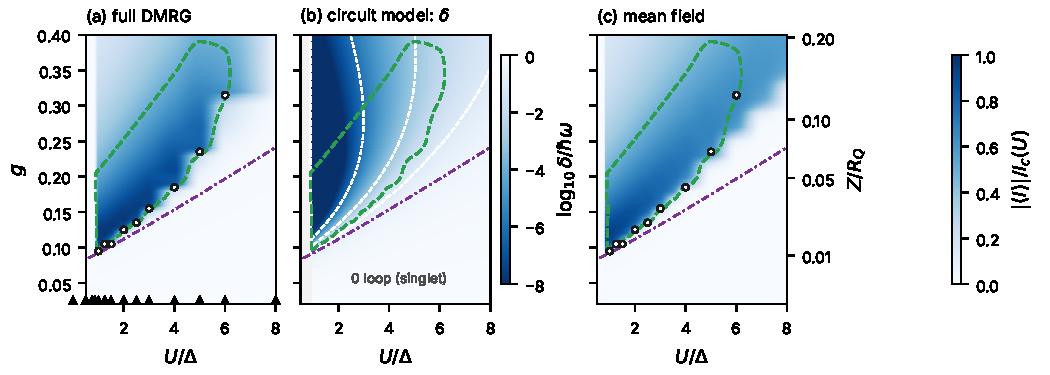
\includegraphics[width=0.9\textwidth]{fig_phase_main.pdf}
  \begin{columns}[T]
    \column{0.34\textwidth}
    \small (a) Full DMRG, 427 ground states, seed $10^{-3}$: persistent current $|\langle I\rangle|/I_c(U)$.
    Triangles: computed $U$; circles: $0.5I_c$.
    \column{0.33\textwidth}
    \small (b) Seed-free order parameter: tunnel splitting $\delta$ of the circuit model with the DMRG $E(\varphi)$.
    Grey: singlet $0$ loop.
    \column{0.33\textwidth}
    \small (c) Mean field (product state). Green dashed: $0.5I_c$ of the circuit model; purple: classical $\beta=1$.
    Right axis: $Z/R_Q$.
  \end{columns}
\end{frame}

% ------------------------------------------------------------------
\begin{frame}{How to read it}
  \begin{columns}[T]
    \column{0.5\textwidth}
    \begin{keybox}[title={$U<U_c$: a $0$ loop}]
      \small Singlet ground state, diamagnetic: the mode is \emph{stiffened}, no current. The boundary moves from
      $0.94\Delta$ to $0.85\Delta$ with $g$: the zero-point flux itself drives a $0\to\pi$ switch.
    \end{keybox}
    \begin{keybox}[title={$U>U_c$, $g>g_c(U)$: the condensate}]
      \small Current $\simeq I_c$, $7$--$9$ photons. $g_c$ follows $\beta=1$ but lies above it by
      $\Delta g=0.02$, $0.04$, $0.12$ at $E_J/\hw=10$, $5$, $3.2$: zero-point motion opposes the condensation.
    \end{keybox}
    \column{0.5\textwidth}
    \begin{keybox}[title={$E_J\lesssim2.5\,\hw$ ($U\gtrsim8\Delta$): no order}]
      \small $\beta$ reaches $2.7$, yet the ground state is the cat, $\delta\simeq\hw$, current $\propto$ seed.
    \end{keybox}
    \begin{warnbox}[title={Mean field (c) fails where it matters}]
      \small Orders at $U=7$--$8\Delta$ with $0.6I_c$ (absent) and at $U=0.85\Delta$ with $0.95I_c$ where the exact state is a
      $0$ loop: a product state cannot be a cat, and replaces the Kramers doublet by a static moment.
    \end{warnbox}
    \small Full DMRG = circuit Hamiltonian to $0.2\%$ of $I_c$: here the loop \emph{is} a $\pi$-fluxonium with the
    microscopic $E(\varphi)$.
  \end{columns}
\end{frame}

% ------------------------------------------------------------------
\begin{frame}{Cuts through the diagram}
  \centering
  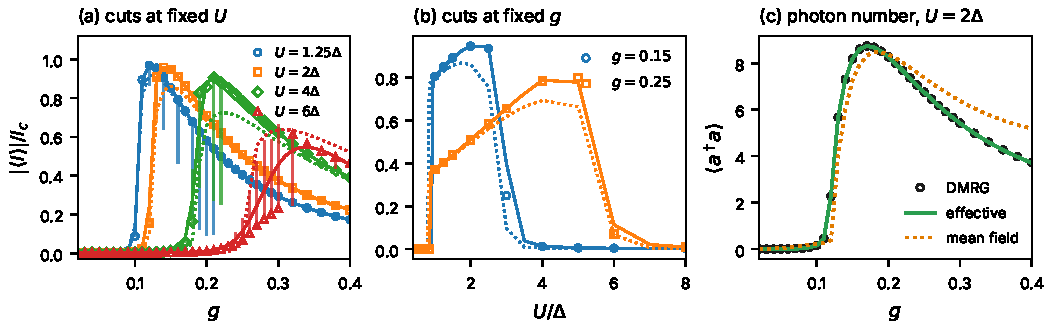
\includegraphics[width=0.95\textwidth]{fig_phase_slices.pdf}
  \par\small Symbols: full DMRG; solid: circuit model; dotted: mean field. The sharp step at $U=1.25$, $2\Delta$
  ($E_J/\hw\simeq13$, $10$) becomes a broad crossover at $U=6\Delta$ ($E_J/\hw=3.2$).
\end{frame}

% ==================================================================
\section{The mean-field approach of the ring notebook, and a caveat}
% ------------------------------------------------------------------
\begin{frame}{The mean-field approach of the ring notebook}
  \begin{columns}[T]
    \column{0.52\textwidth}
    \small Same product-state idea, now for the microscopic ring (\texttt{Optimised\_SC\_ring\_with\_JJ\_cavity\_mean\_field.nb}):
    one dot + $10$ BCS sites ($t_0=2$, $\Delta_0=0.6$, $t_R=t_L=0.5$), the dot \emph{Zeeman-polarized}
    ($\epsilon_\uparrow=-0.3$, $\epsilon_\downarrow=3.7$: a magnetic dot = Hartree--Fock image of a large-$U$ dot),
    one mode $\hbar\omega=0.02$, seed $\varphi_{\rm cl}=10^{-3}$, $g=0$--$1.2$.
    \begin{align*}
      \text{electrons:}&\ \ \text{BdG with the junction bond } t_R\to t_R\,\alpha,\quad \alpha=\langle\psi_{ph}|e^{igX}|\psi_{ph}\rangle\\
      \text{photon:}&\ \ \hbar\omega a^\dagger a-\big(\eta\,e^{igX}+\text{h.c.}\big),\quad
      \eta=t_Re^{i\varphi_{\rm cl}}\langle c^\dagger_1c_0\rangle\\
      E&=E_{\rm el}+E_{\rm ph}+2\,\mathrm{Re}(\eta\alpha),\qquad I=-2\,\mathrm{Im}(\eta\alpha)
    \end{align*}
    \column{0.46\textwidth}
    \begin{keybox}[title={What it predicts}]
      \small A current-carrying phase for $g\gtrsim0.75$: $|I|\approx0.02$, $\langle a^\dagger a\rangle\simeq1$--$1.4$,
      $\langle X\rangle\neq0$ -- the ``photon condensate'' of the circuit model, now from a microscopic ring.
    \end{keybox}
    \begin{keybox}[title={Checks}]
      \small The Python port reproduces all five notebook curves to machine precision; the algebra (Nambu convention,
      double counting, $I=-\partial E/\partial\varphi$) is correct. The question is only the \emph{ansatz}.
    \end{keybox}
  \end{columns}
\end{frame}

% ------------------------------------------------------------------
\begin{frame}{Caveat: with exactly these parameters, DMRG finds nothing -- and why}
  \begin{columns}[c]
    \column{0.36\textwidth}
    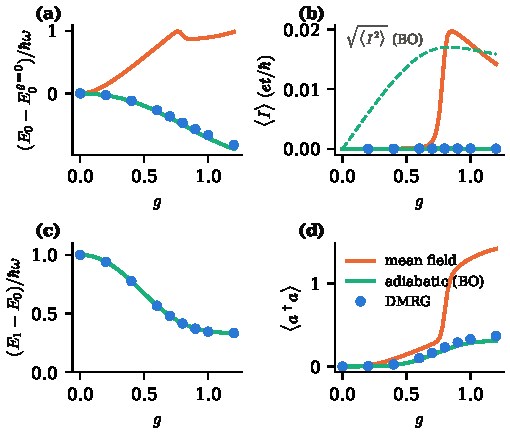
\includegraphics[width=\textwidth]{fig_notebook_model.pdf}
    \column{0.62\textwidth}
    \footnotesize Full DMRG (electrons $\otimes$ photon, same $H$, same seed): \alert{no current} at any $g$, only a linear response
    $7\times10^{-5}$; exact energy $1.8\hbar\omega$ \emph{below} mean field, gap stays $0.33\hbar\omega$, $\langle a^\dagger a\rangle\simeq0.36$.
    The circuit model (exact photon) agrees with DMRG.
    \begin{warnbox}[title={Three reasons}]
      \footnotesize (1) $E_J\simeq\hbar\omega$: the double well ($g>0.58$) is shallower than the zero-point energy; the ground
      state is a cat, which a product state cannot be -- it \emph{self-traps} in one well.\\
      (2) The product state is not gauge covariant: it shrinks the junction bond by $|\langle e^{igX}\rangle|<1$ and loses
      phase-independent kinetic energy that the exact state recovers by following the flux.\\
      (3) $L=11\lesssim\xi$: $E(\varphi)$ is dominated by the $h/e$ harmonic ($E_1=2.1\times10^{-2}\gg E_2=2\times10^{-3}$):
      the ``instability'' would be of the normal persistent current, not of the junction.
    \end{warnbox}
    \footnotesize Same model at $\hbar\omega=0.002$: it \emph{does} order ($g_c=0.21$; mean field $0.30$). The control parameter is
    $E_J/\hbar\omega$ -- hence the manuscript's $E_J/\hbar\omega=10$ and $L\gg\xi$.
  \end{columns}
\end{frame}

% ==================================================================
\section{Outlook}
% ------------------------------------------------------------------
\begin{frame}{Bonus: the vacuum of the mode switches the junction from $0$ to $\pi$}
  \begin{columns}[c]
    \column{0.5\textwidth}
    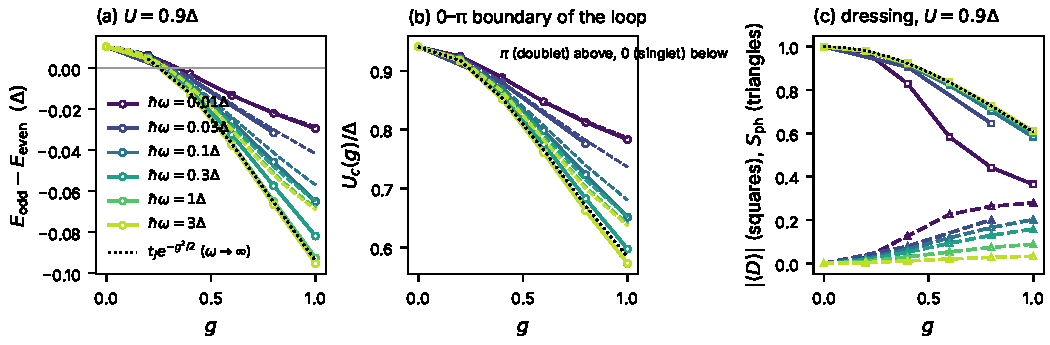
\includegraphics[width=0.78\textwidth,trim=0 0 340 0,clip]{fig_cavity_0pi.pdf}
    \par\small $U=0.9\Delta$: a $0$ junction without the mode becomes a $\pi$ junction at $g\simeq0.3$ ($Z\simeq0.6\,$k$\Omega$).
    \column{0.5\textwidth}
    \begin{itemize}\small
      \item Both parity sectors by full DMRG, no seed, $\hw=0.01$--$3\,\Delta$: $U_c$ of the loop moves down by
            $12\%$ at $g=0.5$ and $30$--$40\%$ at $g=1$.
      \item Slow mode: zero-point flux costs the singlet energy (its surface curves up) and pays the doublet.
            Fast mode: the vacuum average $e^{-g^2/2}$ of the Peierls factor reduces the level width (Franck--Condon).
      \item Observable as the resonator-frequency jump of a gate-tuned dot junction, driven by the impedance alone.
    \end{itemize}
  \end{columns}
\end{frame}

% ==================================================================
\section{Summary}

\begin{frame}{Summary}
  \begin{enumerate}
    \item A $\pi$ junction sharing its inductance with an $LC$ mode is a $\pi$-fluxonium,
          $H=4E_Cn^2+\frac12E_L\theta^2+E_J\cos\theta$: for $\beta=8g^2E_J/\hw>1$ a persistent current and a photon
          condensate appear; the exact ground state is a \alert{cat} of the two current directions.
    \item The \alert{full-DMRG phase diagram} of the microscopic model (dot + BCS ring + photon) confirms it without
          approximation: condensate for $U>U_c$, $g>g_c(U)$; threshold pushed above $\beta=1$ by zero-point motion; no
          order for $E_J\lesssim2.5\,\hw$; mean field fails exactly there and at $U\simeq U_c$.
    \item The zero-point flux of the mode is itself a control parameter of the $0$--$\pi$ transition.
  \end{enumerate}
  \vfill
  \centering Thank you!
\end{frame}

\appendix
\begin{frame}{Backup: physical units}
  \centering\small
  $E_J/h\simeq0.5\,{\rm GHz}\times I_c[{\rm nA}]$, \ $\beta=2\pi(Z/R_Q)(E_J/\hw)$\\[2mm]
  \begin{tabular}{@{}lccccc@{}}
    \toprule
    $U$, $\Gamma$, material & $E_J/h$ & $I_c$ & $E_J/10h$ & $E_J/10k_B$ & $L_{\beta=1}$\\ \midrule
    $2\Delta$, $\Delta/2$, Al & 0.32 GHz & 0.65 nA & 32 MHz & 1.5 mK & 510 nH\\
    $2\Delta$, $\Delta/2$, NbTiN & 2.1 GHz & 4.3 nA & 210 MHz & 10 mK & 76 nH\\
    $6\Delta$, $2\Delta$, NbTiN & 9.9 GHz & 20 nA & 0.99 GHz & 47 mK & 17 nH\\
    $6\Delta$, $2\Delta$, Nb & 11.5 GHz & 23 nA & 1.15 GHz & 55 mK & 14 nH\\ \bottomrule
  \end{tabular}
  \par\vspace{3mm}
  \begin{itemize}\small
    \item Condensate and cat need $E_J/\hw\gtrsim5$ and $\hw>k_BT$: a strong dot junction in NbTiN/Nb with a $\simeq1\,$GHz mode,
          $L\simeq17\,$nH, $Z\simeq160\,\Omega$ (full DMRG: $9.6$ photons, $0.94I_c$).
    \item The flux-driven $0$--$\pi$ switch needs only $\hw=0.03$--$0.3\Delta$ and $Z=0.7$--$3\,$k$\Omega$: Al, $1$--$13$\,GHz, granular-Al superinductors.
  \end{itemize}
\end{frame}

\begin{frame}{Backup: how the current was computed}
  \begin{itemize}
    \item Current operator $I=-(e/\hbar)\partial H/\partial\pcl$ through the dot bond, dressed by $D$; checked against the sum rule
          $\langle I\rangle=(e/\hbar)(\hw/2g)\langle a+a^\dagger\rangle$ at every point (median violation $10^{-4}I_c$).
    \item Seed $\pcl=10^{-3}$ to select a direction; two independent DMRG starts (vacuum side / polarized side) with seed
          annealing, because the two current states are split only by $\delta$ and by $2I^\star\pcl\sim10^{-5}\Delta$.
    \item Seed $10^{-4}$: current unchanged above threshold, reduced $\times0.09$ below -- it is spontaneous.
    \item $\chi=400$ changes energies by $<4\times10^{-8}\Delta$ and the current by $<0.3\%$ away from the crossover.
  \end{itemize}
\end{frame}

\end{document}
